\graphicspath{ {Figures/Pileup/Multiplier/} {Figures/Pileup/Phase/} {Figures/Pileup/EnergyScaling/} {Figures/RandomSeeds/FitStartScans/} {Figures/RandomSeeds/FitIterations/} {Figures/Miscellaneous/} {Figures/FitStartScans/} {Figures/CBO/Frequency/} {Figures/CBO/Shape/} {Figures/CBO/LifetimeScan/} {Figures/Gain/InFill/} {Figures/Gain/InFillCrystals/} {Figures/VW/} {Figures/LostMuons/} {Figures/BunchNumber/} }

\chapter{Systematic Uncertainty Evaluations}
\label{Ch:Systematics}

	As a quick disclaimer, note that not all systematic uncertainty evaluations have been fully completed in this report. In some cases the calculation of only one or two numbers can be improved (eg. the uncertainty of the gain parameters), in others better methods might be developed (eg. the error due to the CBO frequency model used), and still others have been left out entirely (eg. the lost muon bias). These are all a work in progress but the contained results are sufficient for this report.
	

\section{Sensitivity of \texorpdfstring{$\omega_{a}$}{} to gain corrections}
\label{Sec:SystematicGain}

	I estimate the systematic error on R due to the in-fill gain function at 7.2 ppb (including the Short Term Double Pulse correction), and have yet to estimate the error due to solely the SDTP or any other unseen or unknown gain effects. %Adding these in quadrature results in a systematic error of blank ppb.

	\subsection{In-Fill Gain}

		As positrons hit the calorimeters throughout the fill, there will be a gain sag response such that the energy of detected positrons changes throughout the fill. The energy response will drop early in the fill due to the flash and injection of beamline positrons, and then will rise exponentially back up to its static value. This changing energy response will lead to a systematic error on R, as the average \gmtwo phase depends on the energy, and positrons with mis-measured energies near the energy threshold are excluded from the fit. This gain sag is corrected in the Recon West code at the crystal level, before I fill my histograms. The gain correction parameters can be stored at the tree level such that they can be undone and modified for systematic studies.

		The in-fill gain sag function was determined by Matthias Smith and the laser team as described in \DB{14077}. The function goes as  
			\begin{gather}
				E = E_{0}(1 - A \cdot e^{-t/\tau}),
			\label{Eqn:GainSag}
			\end{gather}
		where $E$ is the corrected energy of the crystal hit, $E_{0}$ is the original energy of the crystal hit, A is the amplitude factor on the gain sag function, and $\tau$ the lifetime. $E/E_{0}$ is shown in Figure \ref{Fig:MatthiasInFill}. It is this function that is inverted and applied to the crystal hits in the reconstruction, before adding the individual crystal energies to form the clusters. For these systematic studies, I undo this function on each crystal before reapplying it with varying amplitude and lifetimes. In this way I can scan over multipliers of the amplitude and lifetime parameters in order to calculate the systematic effect on R.

		\begin{figure}[h]
			\centering
			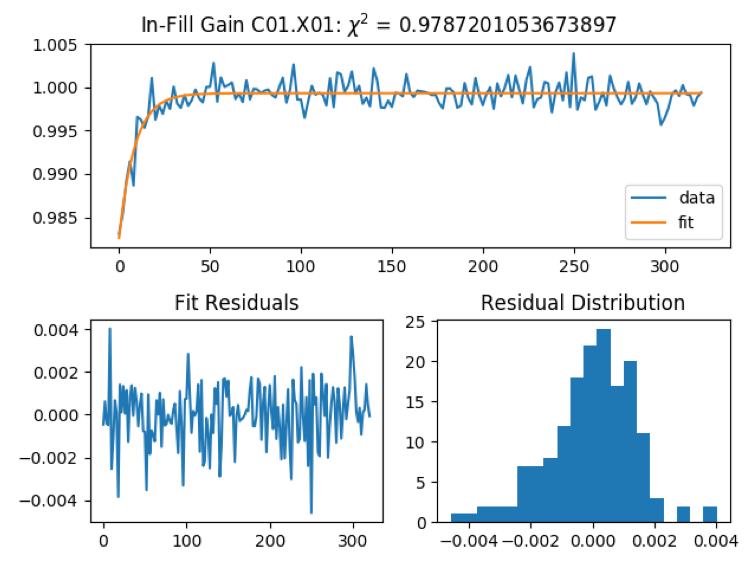
\includegraphics[width=.8\textwidth]{MatthiasInFill}
		    \caption[MatthiasInFill]{The top plot shows the in-fill gain sag function in orange from a fit to data in blue, for crystal 1 in calorimeter 1. The gain sag can be modeled effectively by a simple exponential function. By $\SI{30}{\mu s}$ the change in energy response is nearly only .1\%. The bottom two plots show the residuals of the fit. Plot made by Matthias Smith.}
		    \label{Fig:MatthiasInFill}
		\end{figure}

		For the error due to the amplitude, I applied multipliers on the amplitude of 0, 0.9, 0.95, 1, 1.05, 1.1, and 2. For the error due to the lifetime, I applied multipliers of 0.1, 0.9, 0.95, 1, 1.05, 1.1, and 2. The results of these scans are shown in Figure \ref{Fig:InFillGain}. I included the mulipliers of 0 (or 0.1) and 2 in order to calculate outer limits on the error. The multipliers of 2 resulted in a 7 ppb change on R due to the amplitude, and an 85 ppb change due to the lifetime. The change in R due to the multipliers of 0 or 0.1 were 6 ppb due to both the amplitude and lifetime. I calculate the systematic error on R as the quadrature sum of the separate pieces: 
		\begin{align}
			\delta R_{A} &= \delta\alpha_{A} \times \frac{dR}{d\alpha_{A}}, \\
			\delta R_{\tau} &= \delta\alpha_{\tau} \times \frac{dR}{d\alpha_{\tau}},
		\end{align}
		where $\delta\alpha_{A}$ and $\delta\alpha_{\tau}$ are the uncertainties on the gain sag amplitude and lifetime respectively. I assume that these errors are uncorrelated. I take the uncertainties on the amplitude and lifetime at 10\%. This leads to systematic errors on R of $0.1 \times \SI{57.9}{ppb} = \SI{5.8}{ppb}$ and $0.1 \times \SI{42.9}{ppb} = \SI{4.3}{ppb}$ respectively. In each of these cases, the uncertainty is the uncertainty on the applied parameters, and not the stability or precision of the energy response over the course of the fill. These added in quadrature results in a systematic error on R of 7.2 ppb.

		\begin{figure}[]
		\centering
		    \begin{subfigure}[t]{0.45\textwidth}
			    \centering
				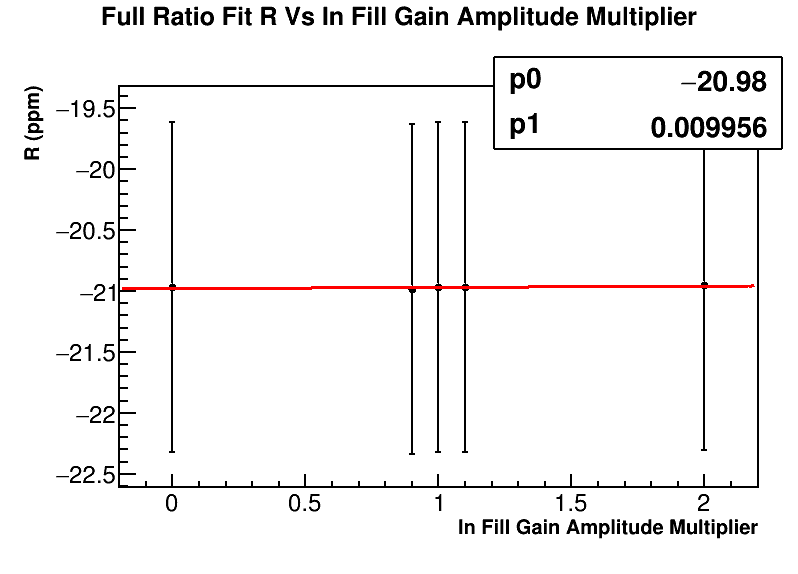
\includegraphics[width=\textwidth]{R_Vs_IFG_Amp_crystals}
			    \caption{Plotted is R vs the multiplier on the amplitude parameter in the gain sag function. A greater slope was observed when exluding the outer points, by over an order of magnitude. In order to be conservative I fit just the inner points. The slope is 57.9 ppb per unit amplitude.}
		    \end{subfigure}
		    \hspace{4mm}
		    \begin{subfigure}[t]{0.45\textwidth}
			    \centering
				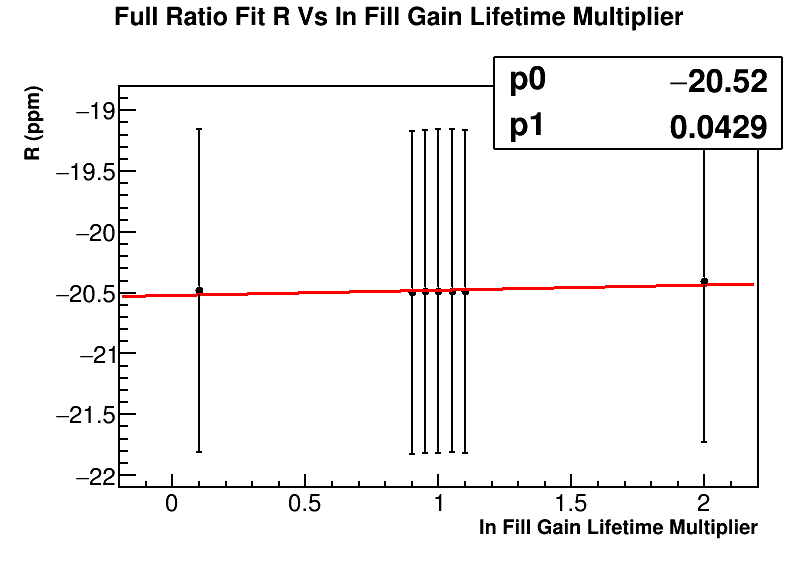
\includegraphics[width=\textwidth]{R_Vs_IFG_Tau_crystals}
			    \caption{Plotted is R vs the multiplier on the lifetime parameter in the gain sag function. The slope is 42.9 ppb per unit lifetime.}
		    \end{subfigure}% %you need this % here to add spacing between subfigures
		\caption[InFillGain]{Plotted are the fitted R values vs gain sag function parameter multipliers. In each case, these parameter multipliers were applied to each crystal individually, after undoing the gain sag correction done in the reconstruction. The fact that the outer points change the R value by so little indicates that the ratio fit is largely insensitive to the amplitude and lifetime of the gain function, as it is divided out.}
		\label{Fig:InFillGain}
		\end{figure}


	\subsection{Short Term Double Pulse (SDTP)}

		To determine the systematic effect from the SDTP correction, the path forward is to reconstruct the cluster with and without the correction and observe the change in R. I expect it to be small considering how small the in fill gain systematic error was.

	\subsection{Unseen/Unknown Gain Changes}

		More thought needs to be given on how any unseen gain changes might affect R.

\section{Sensitivity of \texorpdfstring{$\omega_{a}$}{} to pileup}
\label{Sec:SystematicPileup}

	The systematic error on R due to the pileup construction consists primarily of two parts, the error due to misconstruction of the amplitude and the phase of the pileup. I estimate the systematic error on R due to the pileup amplitude at 24.1 ppb, and to the pileup phase in pieces of 23.1 and 17.1 ppb. Adding these in quadrature results in a systematic error of 37.5 ppb.

	\subsection{Pileup Amplitude}

		The error due to the amplitude misconstruction was calculated by scanning over a pileup multiplier parameter, from 90\% of the calculated pileup amplitude to 110\%, as shown in Figure \ref{fig:PileupMultiplier}. The sensitivity of R to the amplitude was determined to be -553.4 ppb per unit amplitude. The uncertainty of the pileup amplitude construction was determined by fitting a parabola to the \chisq as a function of the pileup amplitude, and taking the width of that parabola as the uncertainty. This width is determined as the distance in X for the \chisq to rise by 1 from the minimum, also calculated as $\sqrt{2/(\chi^{2})''}$.

		\begin{figure}[h]
		\centering
		    \begin{subfigure}[t]{0.45\textwidth}
			    \centering
				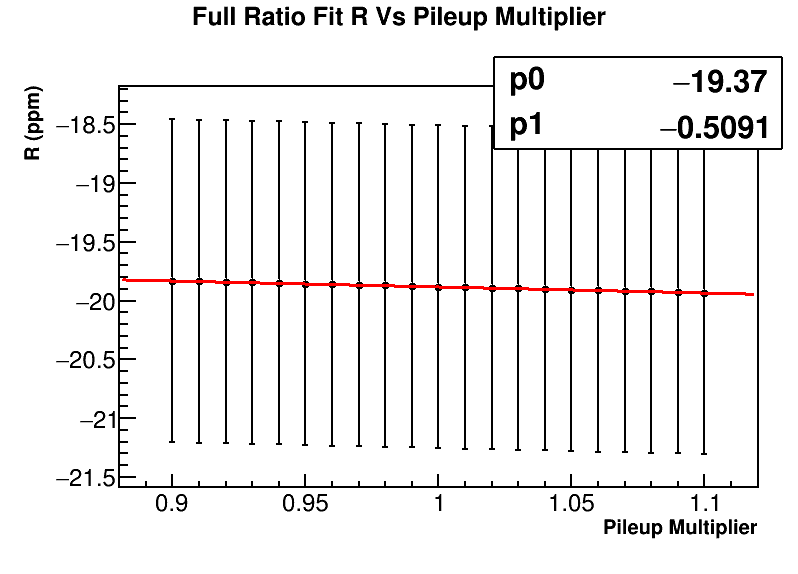
\includegraphics[width=\textwidth]{RatioCBO_R_Vs_PileupMultiplier_Canv}
			    \caption{Sensitivity of R vs the pileup amplitude. The slope is -553.4 ppb per unit amplitude.}
		    \end{subfigure}
		    \hspace{4mm}
		    \begin{subfigure}[t]{0.45\textwidth}
			    \centering
				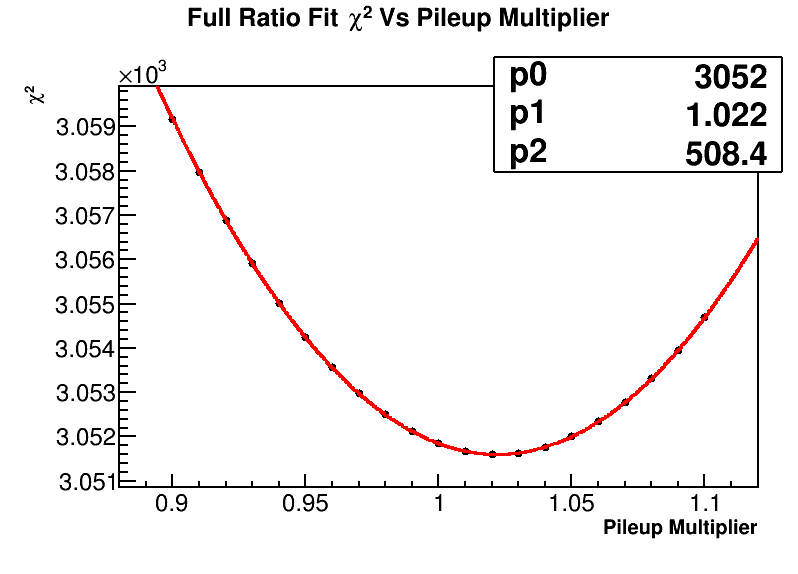
\includegraphics[width=\textwidth]{RatioCBO_Chi2_Vs_PileupMultiplier_Canv}
			    \caption{Plotted is the fitted \chisq vs the pileup amplitude. The fit equation used was $p2 \times (x - p1)^{2} + p0.$ The minimum lies at 0.9993.}
		    \end{subfigure}
		\caption[PileupMultiplier]{The significant plots to determine the pileup amplitude systematic error.}
		\label{fig:PileupMultiplier}
		\end{figure}

		This corresponds to an uncertainty of $\sqrt{1/526.5} = 0.0436$ or 4.36\%. The minimum of the \chisq plot is consistent with 1. (Note that this minimum flucuates with the random seed, and simply needs to be statistically consistent with 1). Then, calculating the systematic error on R due to the pileup amplitude construction as 
			\begin{align}
				\delta R_{pm} = \delta\alpha_{pm} \times \frac{dR}{d\alpha_{pm}}
			\end{align}
		where $\delta\alpha_{pm}$ is the uncertainty on the pileup amplitude, the systematic error on R is calculated as $0.0436 \times \SI{553.4}{ppb} = \SI{24.1}{ppb}$.

		Another technique to estimate the uncertainty of the pileup amplitude construction is to look at the offset of the high energy tail of the pileup subtracted energy spectrum from zero. Because however I've applied only the doublet correction, I know that the shape of the pileup spectrum is wrong by some amount, as evidenced in Figure \ref{fig:AddedEnergies}. While the pileup itself can multiplied by some scaling factor other than 1 in order to align the energy spectra slightly better, because the shape of the pileup correction is imperfect the offset calculation I believe is the wrong way to go about calculating this uncertainty in my case. The shape can be fixed by including the triplets and the doublet contamination in the shadow method, but that work is incomplete. Since the triplets are a 1\% effect relative to the doublets, and the contamination is of the same order, I believe the uncertainty of 4.36\% conservatively includes for this mismatch in shape and the omission of the triplets. Regardless, since the statistics of the 60H dataset is much larger than the order of the systematic effect for the pileup construction ($\mathcal{O}$(1 ppm) vs $\mathcal{O}$(10 ppb)), this is a fine assumption.

	\subsection{Pileup Phase}
	\label{SubSec:PileupPhase}

		The error on R due to the pileup phase construction was calculated by scanning over a pileup time shift parameter, where the pileup spectrum was shifted in time by some amount before subtraction. The sensitivity of R to this parameter is shown in Figure \ref{fig:PileupPhase}. It is unlikely that the entire pileup spectrum could be shifted by the offsets shown here, so this is a conservative estimate of the effect of the pileup phase on R. I then calculate the phase error as 
			\begin{align}
				\delta R_{pp} = \delta\alpha_{pp} \times \frac{dR}{d\alpha_{pp}}
			\end{align}
		where $\delta\alpha_{pp}$ is the uncertainty on the pileup phase. Conservatively estimating the uncertainty on the pileup phase as half the artificial deadtime at 3 ns, the systematic error on R is then calculated as $\SI{3}{ns} \times \SI{7.697}{ppb/ns} = \SI{23.1}{ppb}$. Figure \ref{fig:PileupTimeShiftFS} shows the change in R vs fit start times for pileup time shifted spectra vs the unshifted pileup time spectra. As shown the difference converges to zero as the level of pileup diminishes over the course of a fill.

		\begin{figure}[]
			\centering
			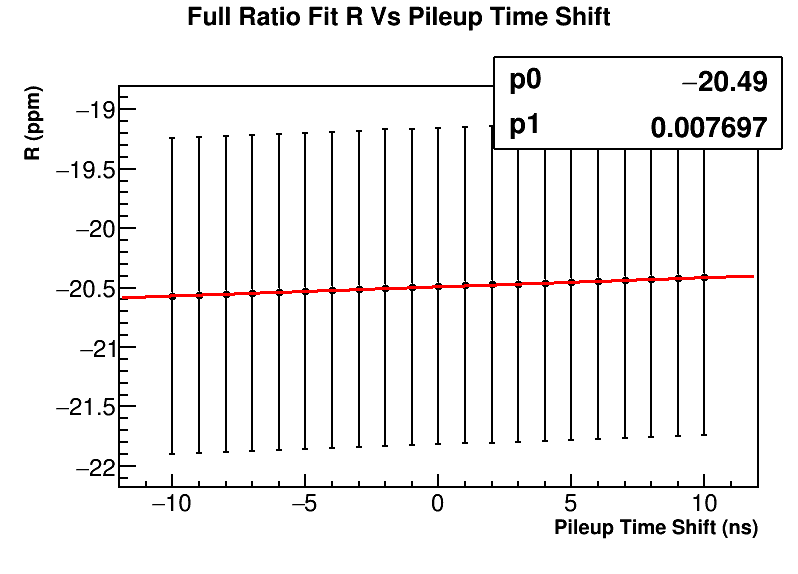
\includegraphics[width=.5\textwidth]{RatioCBO_R_Vs_PileupTimeShift_Canv}
		    \caption[PileupPhase]{Sensitivity of R vs the pileup phase. The slope is 7.697 ppb per ns.}
		    \label{fig:PileupPhase}
		\end{figure}

		\begin{figure}[]
			\centering
			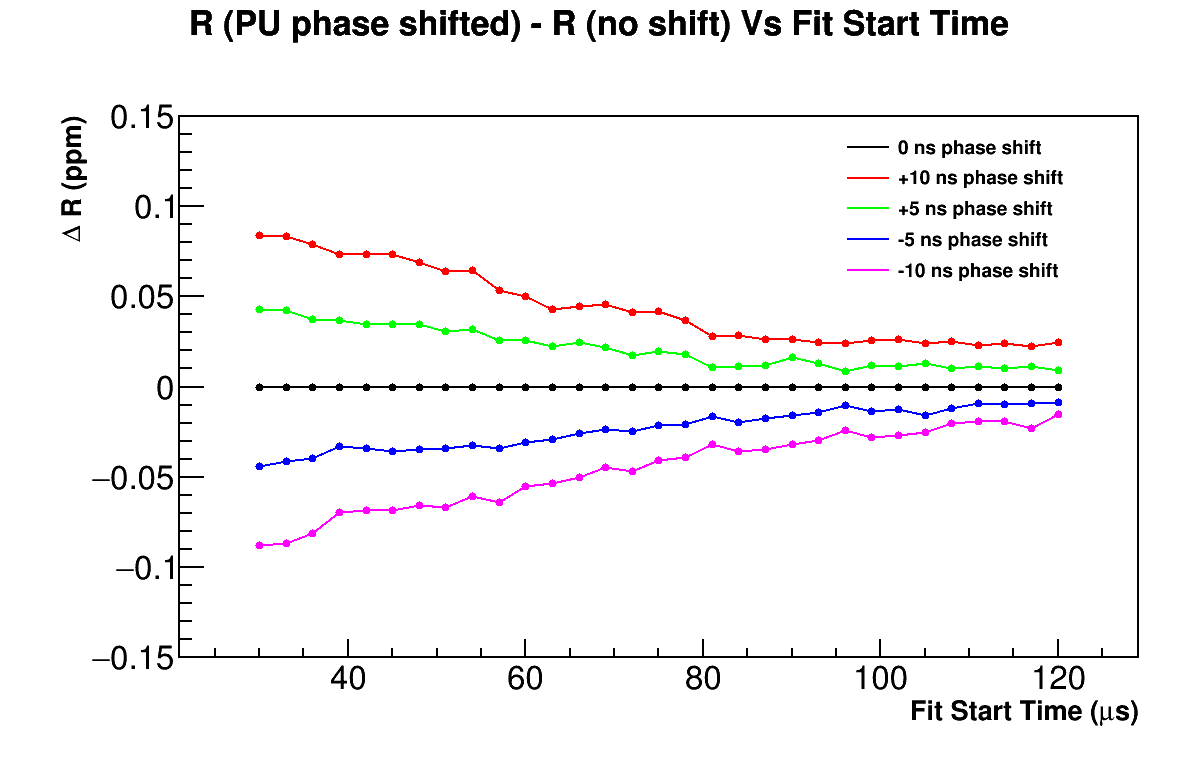
\includegraphics[width=.8\textwidth]{pileupTimeShiftComparison}
		    \caption[PileupTimeShiftFS]{Plotted is $\Delta R$ between pileup time shifted and unshifted results vs fit start time. The black line and points are by definition 0. As the fit start time increases and the pileup reduces, the $\Delta R$ points converge to zero as they should. Plot created on 5033A dataset.}
		    \label{fig:PileupTimeShiftFS}
		\end{figure}

		As mentioned in section Section \ref{Sec:PileupCorrection}, the energy of the pileup pulses may not actually be exactly equal to the sum of the pileup singlets. If the energy of the pileup pulses are systematically miscalculated, then doublets will be added or lost near the energy threshold applied when constructing the pileup spectrum. This leads to an additional error on the phase which needs to be included. With the energy of the pileup pulses calculated as
			\begin{align}
				E_{doublet} = C \cdot (E_{1} + E_{2}),
			\end{align}
		by scanning over the parameter C this error can be determined. The sensitivity of R to this pileup energy scaling parameter is shown in Figure \ref{fig:PileupEnergyScaling}, with a slope of -841.6 ppb per unit scaling parameter. The systematic error on R is calculated in the usual way,
			\begin{align}
				\delta R_{pe} = \delta\alpha_{pe} \times \frac{dR}{d\alpha_{pe}}
			\end{align}
		where $\delta\alpha_{pe}$ is the uncertainty on the pileup energy dependence. This uncertainty was calculated in the same manner as was done for the pileup amplitude, by fitting a parabola to the \chisq as a function of the energy scaling parameter, and it was determined to be 2.03\%. The systematic error on R is then calculated as $0.0203 \times \SI{841.6}{ppb} = \SI{17.1}{ppb}$.

		\begin{figure}[]
		\centering
		    \begin{subfigure}[t]{0.45\textwidth}
			    \centering
				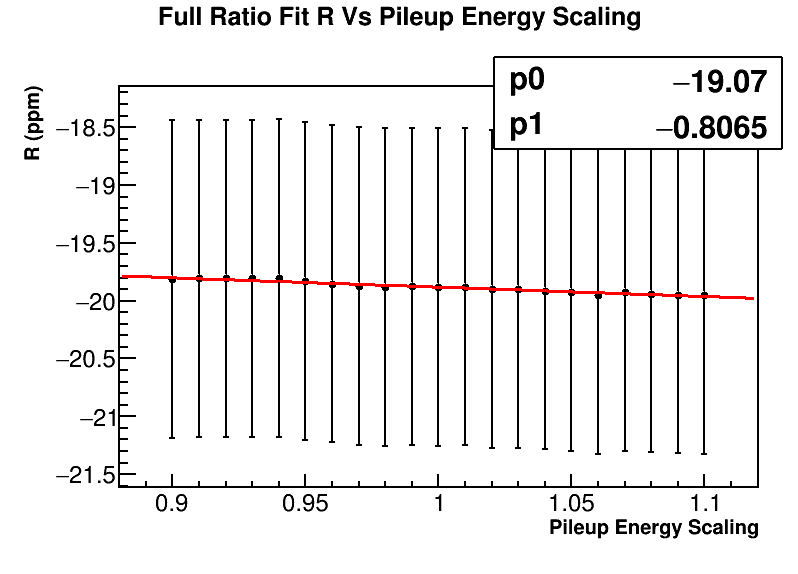
\includegraphics[width=\textwidth]{RatioCBO_R_Vs_PileupEnergyScaling_Canv}
			    \caption{Sensitivity of R vs the pileup energy scaling parameter. The slope is -841.6 ppb per unit energy scaling.}
		    \end{subfigure}
		    \hspace{4mm}
		    \begin{subfigure}[t]{0.45\textwidth}
			    \centering
				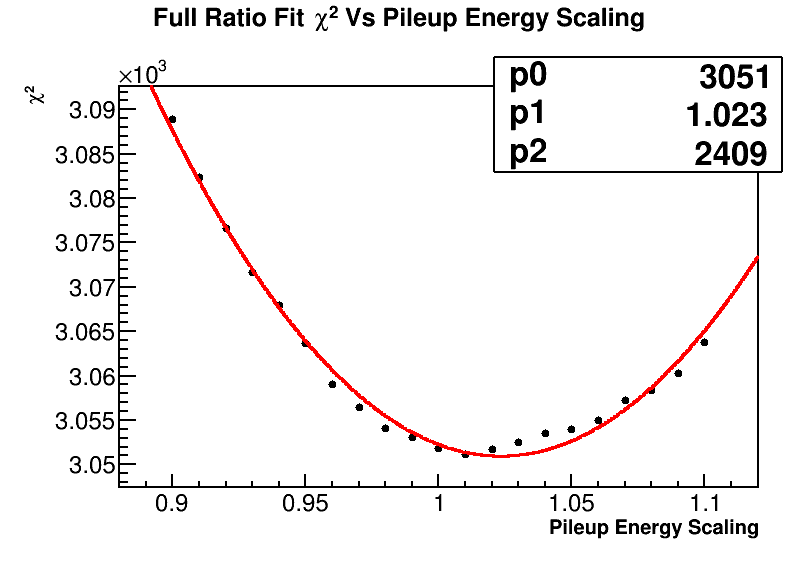
\includegraphics[width=\textwidth]{RatioCBO_Chi2_Vs_PileupEnergyScaling_Canv}
			    \caption{Plotted is the fitted \chisq vs the pileup energy scaling parameter. The fit equation used was $p2 \times (x - p1)^{2} + p0.$ The minimum lies at 1.013.}
		    \end{subfigure}
		\caption[PileupEnergyScaling]{The significant plots to determine a part of the pileup phase systematic error.}
		\label{fig:PileupEnergyScaling}
		\end{figure}


\section{Sensitivity of \texorpdfstring{$\omega_{a}$}{} to lost muons}
\label{Sec:SystematicLM}

	I estimate the systematic error on R due to the lost muon function at 29.9 ppb, and have yet to estimate the systemetic error due to the lost muon bias.

	\subsection{Lost muon function}
	\label{SubSec:LMFunc}

		As described in Section \ref{Sec:LM}, the lost muon function does not need to be included in the ratio fit. In order to calculate a systematic error from excluding the lost muon function, I added the function to the fit as described in that section. I fixed the value of the $\kappa_{loss}$ parameter to that determined from a T Method fit of the same data. The results can be seen in Figure \ref{fig:LMModuloPlot}. The final fitted R value differs from the non-LM fitted function by -29.9 ppb. Therefore I take the the systematic error from excluding the lost muon function as 29.9 ppb.

		\begin{figure}[]
			\centering
			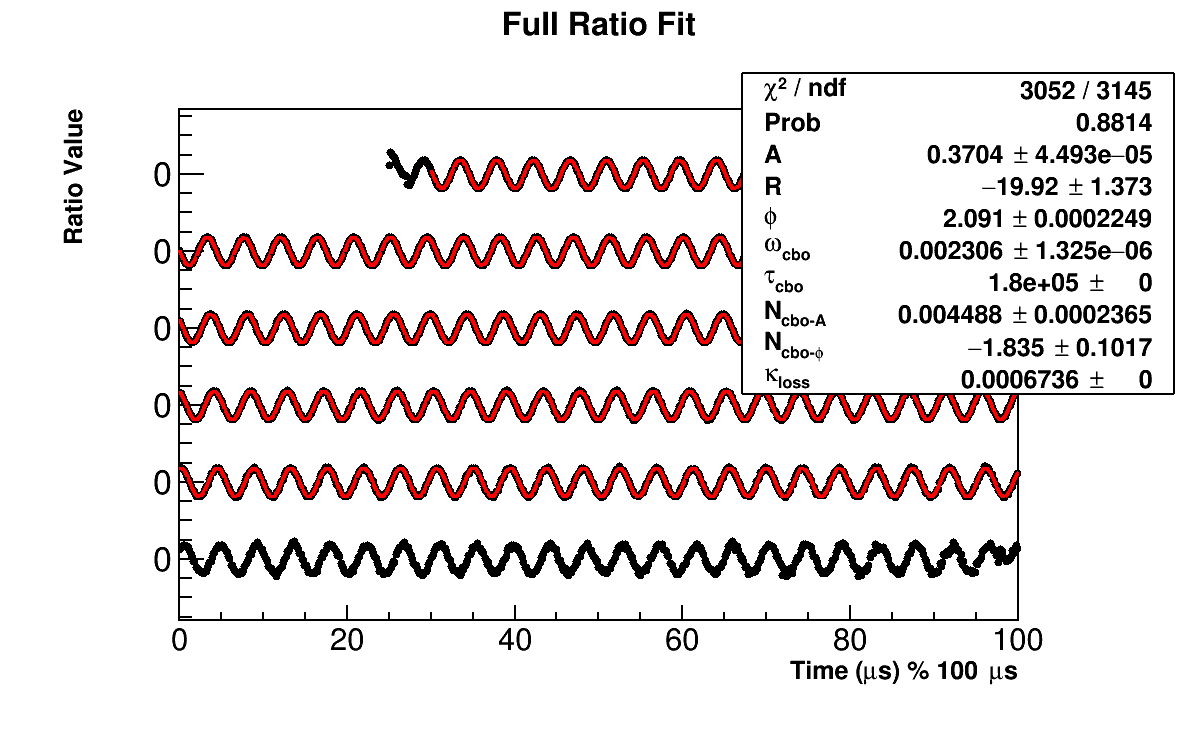
\includegraphics[width=\textwidth]{ratioCBO_moduloPlot-lostmuonsfixed}
		    \caption[LMModuloPlot]{Fit results with the LM term included. The lost muon parameter has been fixed. The x axis is in units of $\mu$s modulo 100 $\mu$s, with successive portions of the data points and fit shifted downwards on the plot. The fit ranges from $\SI{30.2}{\mu s}$ to $\SI{650}{\mu s}$.}
		    \label{fig:LMModuloPlot}
		\end{figure}


	\subsection{Lost muon bias}

		If lost decay positrons (from lost muons) have different average \gmtwo phases than the measured decay positrons, there will be a changing \gmtwo phase over the course of a fill. This will produce a systematic effect on R, pulling its value. A study of this effect is beyond the scope of this report, and will be left out. However it should be noted that this error is likely sizeable, $\mathcal{O}(100)$ ppb or so.


\section{Sensitivity of \texorpdfstring{$\omega_{a}$}{} to CBO function}
\label{Sec:SystematicCBO}

	Results produced on the 5033A dataset. \\

	I estimate the systematic error on R due to the CBO frequency at 30 ppb, to the CBO envelope shape at 21.1 ppb, and to the fixed CBO lifetime at 12.1 ppb. Adding these in quadrature results in a systematic error of 38.6 ppb.

	\subsection{CBO Frequency}
	\label{Sec:CBOFreq}

	As described in Section \ref{Sec:CBO}, the CBO frequency as a function of time changes over the course of a fill. Shown in Figure \ref{fig:CBOFreqModel} is a comparison between the fitted CBO frequency parameter as a function of fit start time for a constant frequency vs a changing frequency. Without the changing frequency the fit behaves improperly. Because a specific model was chosen for the CBO frequency, there will be a systematic error on R that needs to be determined. James Mott examined the frequency function he derived from the data in greater detail in \DB{15376}, where he considered parameter correlations in Equation \ref{Eqn:CBOFreq} and subsequent effects on the overall function. He found that errors were small, parameters were highly correlated, and that the CBO frequency function was very well constrained, as well as comparable between stations 12 and 18, and the 60H and 9d datasets. 

	In order to determine the systematic error on R, I simply varied the individual fixed parameters in the CBO frequency function $\{\Delta\omega, A, \tau_{A}, B, \tau_{B}\}$, by $\pm 2 \sigma$, where the errors on the parameters were taken from \DB{15376}. I also fit the data with the station 18 parameters. Even though the frequency parameters are highly correlated, varying them individually should be a conservative method for determining the overall systematic error on R. I found a 25 ppb difference in the fitted R value for the station 18 parameters, as compared to the station 12 parameters, primarily due to the different ``A'' value, and differences of order 5 ppb or less for the rest of the parameters. Adding them in quadrature resulted in an error of approximately 27.3 ppb. In order to be slightly more conservative, I estimate the systematic error on R due to the frequency at 30 ppb.

		\begin{figure}[]
		\centering
		    \begin{subfigure}[t]{0.45\textwidth}
			    \centering
				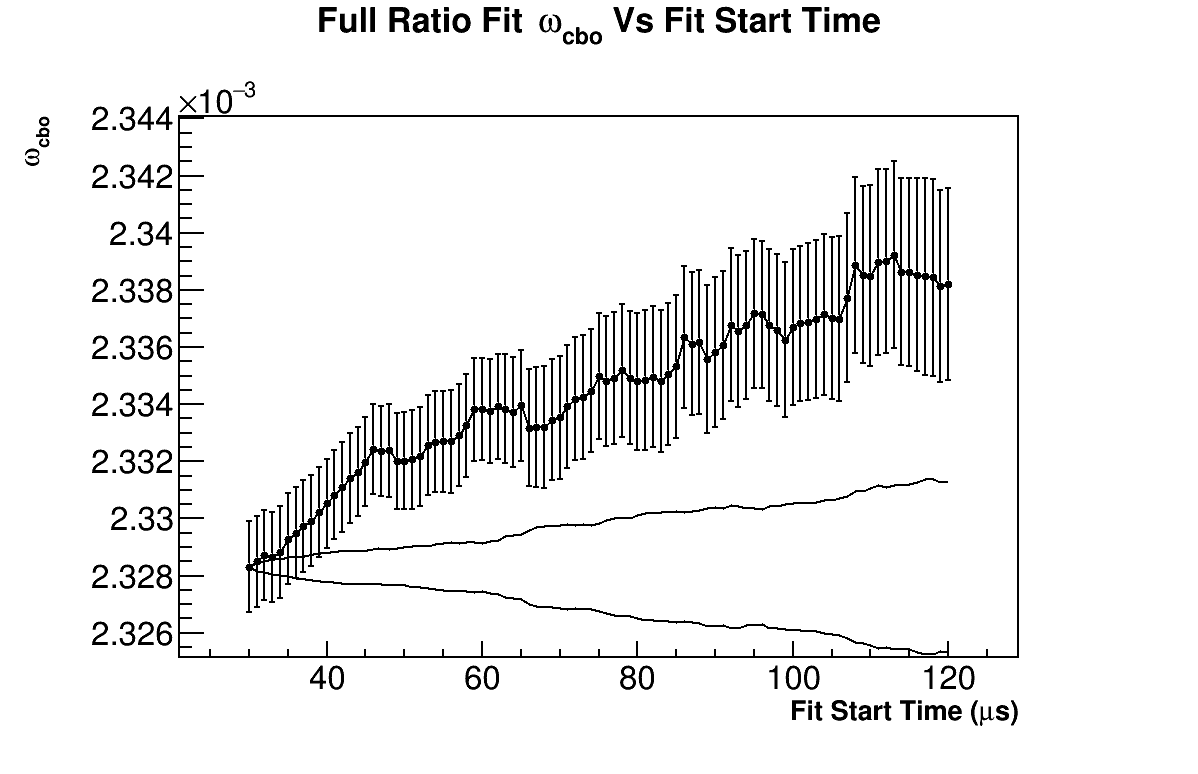
\includegraphics[width=\textwidth]{fixed-wcbo-vs-fs}
			    \caption{Fixed CBO frequency.}
		    \end{subfigure}
		    \hspace{4mm}
		    \begin{subfigure}[t]{0.45\textwidth}
			    \centering
				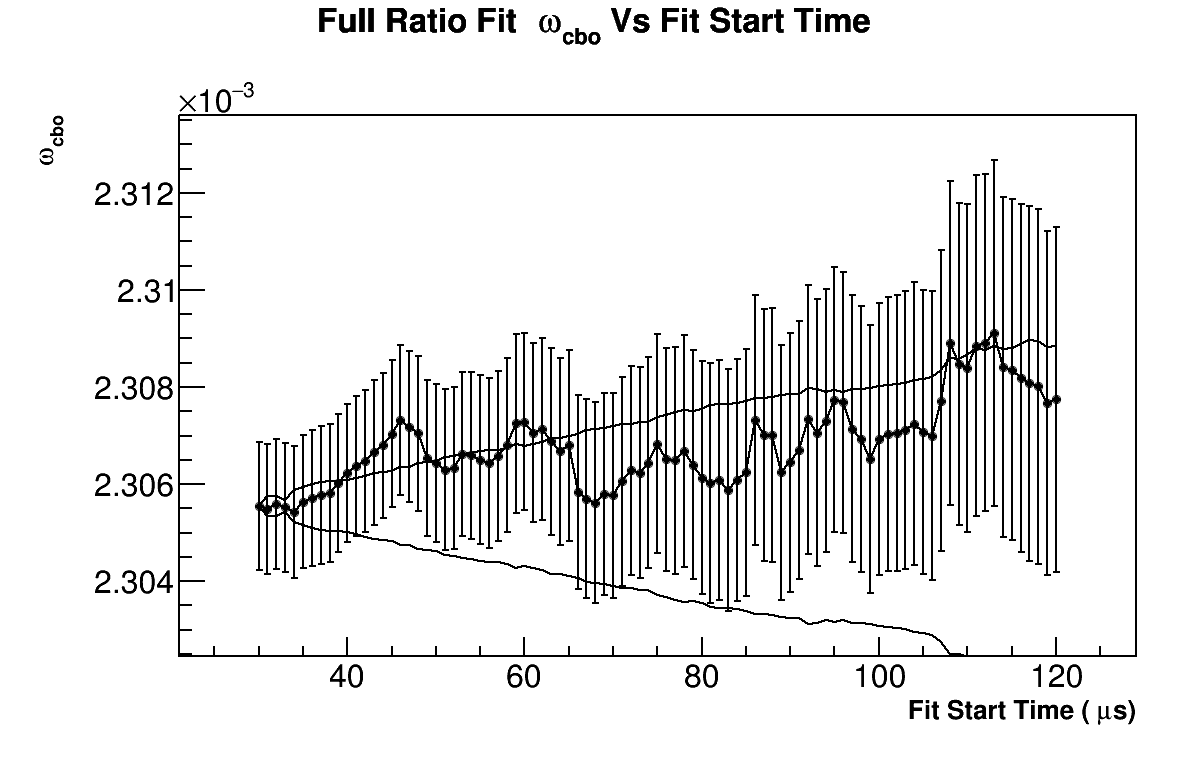
\includegraphics[width=\textwidth]{RatioCBO_omega_cbo_FS_Canv}
			    \caption{Changing CBO frequency.}
		    \end{subfigure}
		\caption[CBOFreqModel]{Fit start time scans for the CBO frequency parameter with a fixed frequency (left) and for the tracker model frequency (right). With the inclusion of the changing frequency over time, the fit parameter becomes stable as a function of fit start time. (Note that the plot on the left was produced with the 5033A dataset, and the fitted parameter was in different units at the time of creation.)}
		\label{fig:CBOFreqModel}
		\end{figure}


	\subsection{CBO Shape}
	\label{SubSec:CBOShape}

		If the shape of the CBO in the fit function is wrong, then there will be a systematic error on R. Because I get good fits and the CBO parameters are stable vs fit start time, the possbile changes to the envelope are limited, compared to the envelope used as shown in Equation \ref{eqn:CBO}. Possible changes to the envelope include those functions as shown in Figure \ref{fig:CBOShapeAmplitude}, an exponential plus a constant and then an exponential times another oscillatory term. Both new envelopes were determined from tracker analysis fits to the CBO amplitude. Both changes to the envelope amplitude were tried in the fitting function, with changes in R of $\SI{-21.1}{ppb}$ and $\SI{-9.6}{ppb}$ respectively, though neither showed any improvement in the fit. (In the latter the period of the oscillatory term was fixed and the other parameters were allowed to float.) I take the latter value of $\SI{21.1}{ppb}$ as the systematic error on R due to the shape.

		\begin{figure}[]
			\centering
			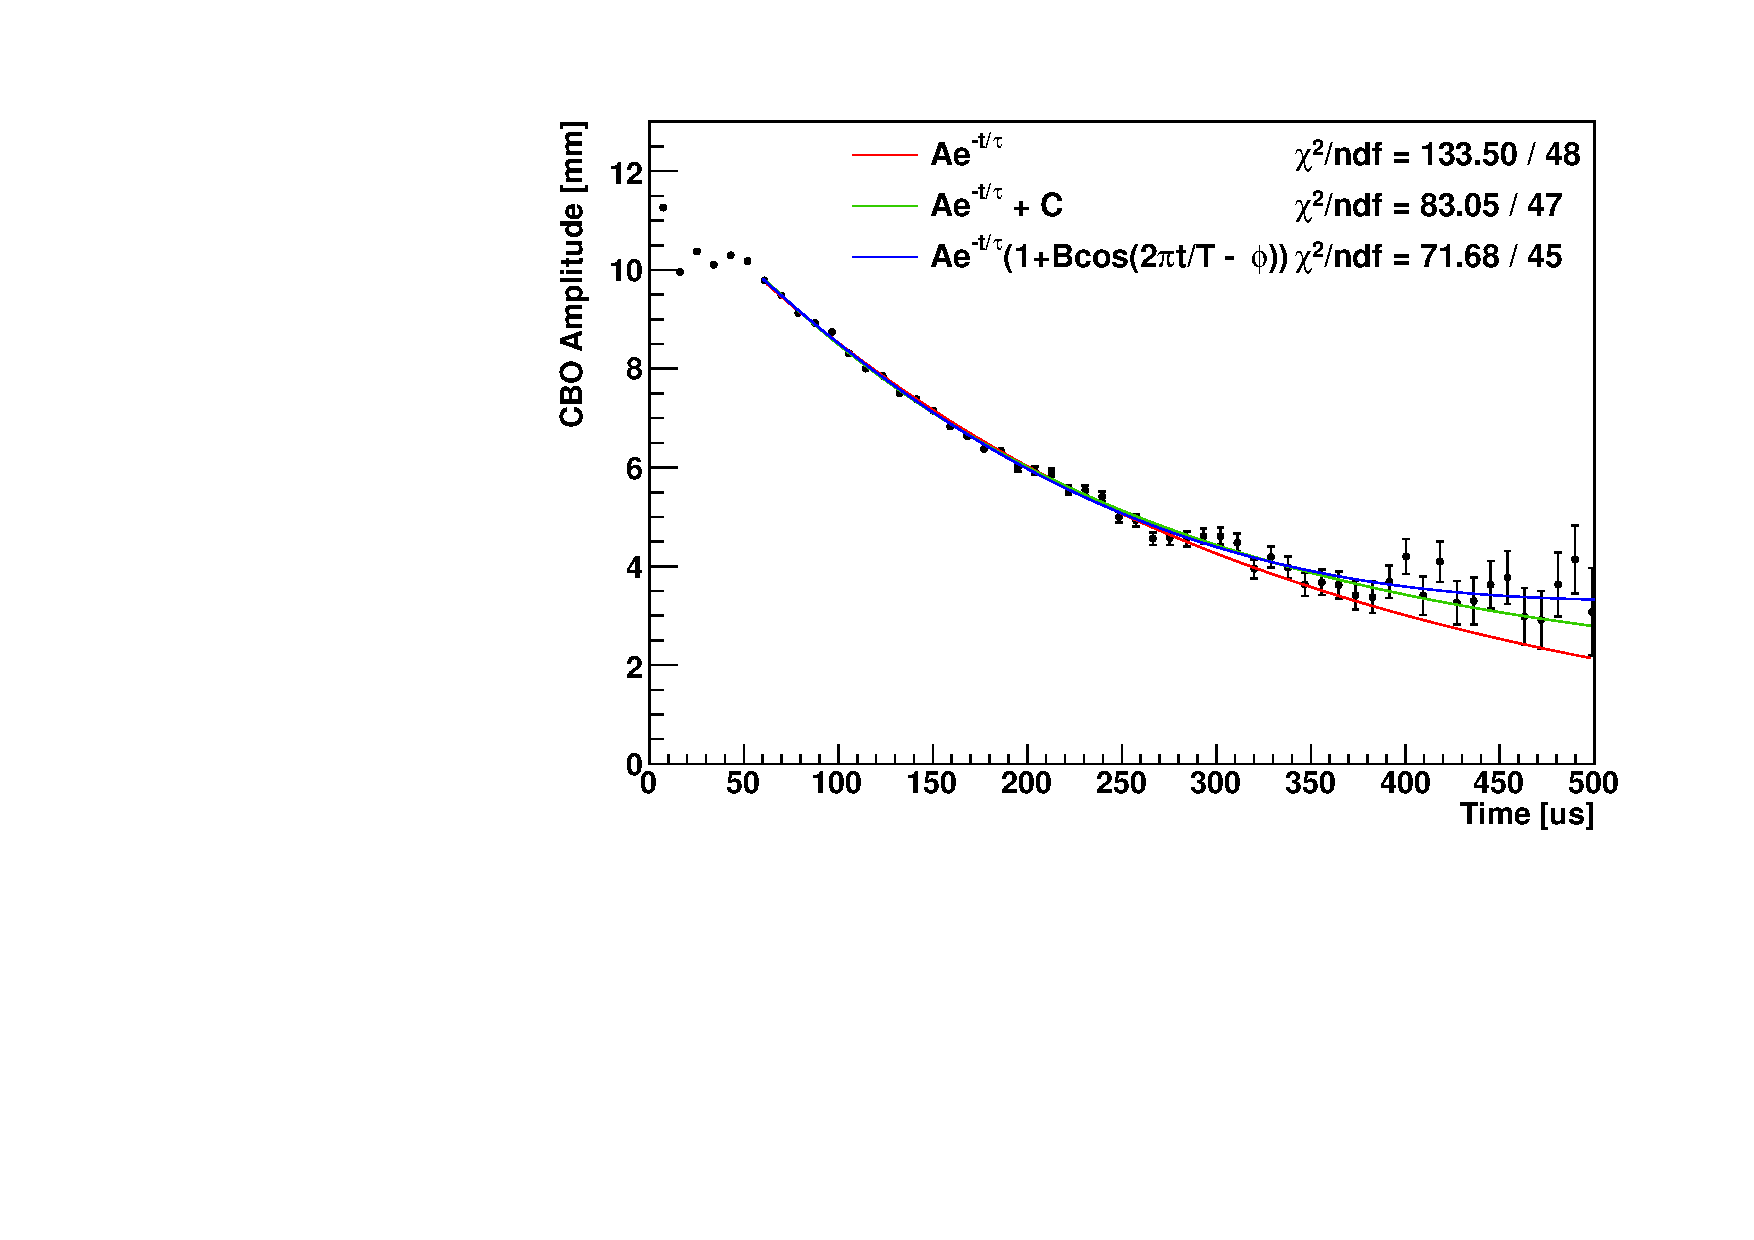
\includegraphics[width=.7\textwidth]{AmplFitOptions}
		    \caption[CBOShapeAmplitude]{Plotted is the CBO amplitude as a function of time from the tracker analysis. Three separate fit functions were used with varying degrees of success to characterize the envelope shape of the CBO (excepting the cosine modulation part). A Gaussian fit was tried with no success. The amplitude isn't fully understood at early times. The period T/$2\pi$ has a value of $\SI{114.5}{\mu s}$. Plot producd by James Mott.}
		    \label{fig:CBOShapeAmplitude}
		\end{figure}

	\subsection{CBO Lifetime}

		I plan on removing this systematic when refitting new dataset, with the cbo lifetime floating. \\

		Because the CBO lifetime has been fixed in the fit, there is a systematic error on R. Scanning over various values of the fixed CBO lifetime allows this error to be calculated. The resulting curve of R vs the CBO lifetime turns out not to be linear, as shown in Figure \ref{fig:CBOLifetime}. Taking the uncertainty on the CBO lifetime as the error produced by the T Method fit, approximately $\SI{16}{\mu s}$, and looking at the change in R for CBO lifetime values of $180 \pm \SI{16}{\mu s}$, the systematic error on R is taken as the larger of the two at 12.1 ppb.

		\begin{figure}[]
			\centering
			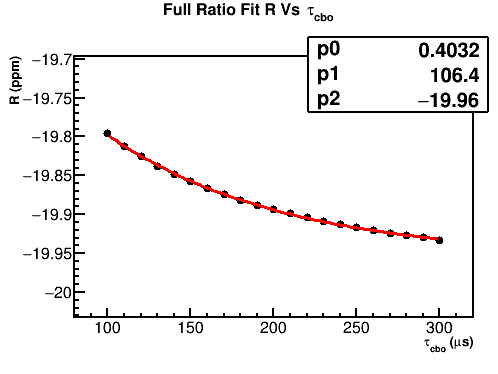
\includegraphics[width=.6\textwidth]{RatioCBO_R_Vs_tau_cbo_Canv}
		    \caption[CBOLifetime]{Plotted is the fitted R value as a function of the CBO lifetime, which has been fixed in the full ratio fit. The error bars have been removed from the plot in order to show the shape of the curve better. The points have been fitted to an exponential function which lines up nicely, $p_{0} e^{-t/p_{1}} + p_{2}$.}
		    \label{fig:CBOLifetime}
		\end{figure}

	\subsection{CBO Fit Terms}
	\label{SubSec:CBOFitTerms}

		I plan on estimating a systematic error due to excluded CBO terms (like the CBO phase term) with the new dataset.



\section{Sensitivity of \texorpdfstring{$\omega_{a}$}{} to VW function}
\label{Sec:SystematicVW}

	As described in Section \ref{Sec:VW}, the vertical waist does not need to be included in the ratio fit. In order to calculate a systematic error from excluding the VW, I added the VW to the fit as described in that section, with an exponentially decaying cosine term. Since the fit is unstable in regards to the amplitude and lifetime parameters, I fixed them to values determined from a T Method fit of the same data. The results can be seen in Figure \ref{fig:VWModuloPlot}. The final fitted R value differs from the non-VW fitted function by less than 1 ppb. This is unsurprising since I'm trying to fit an effect which does not exist in the ratio.

	\begin{figure}[]
		\centering
		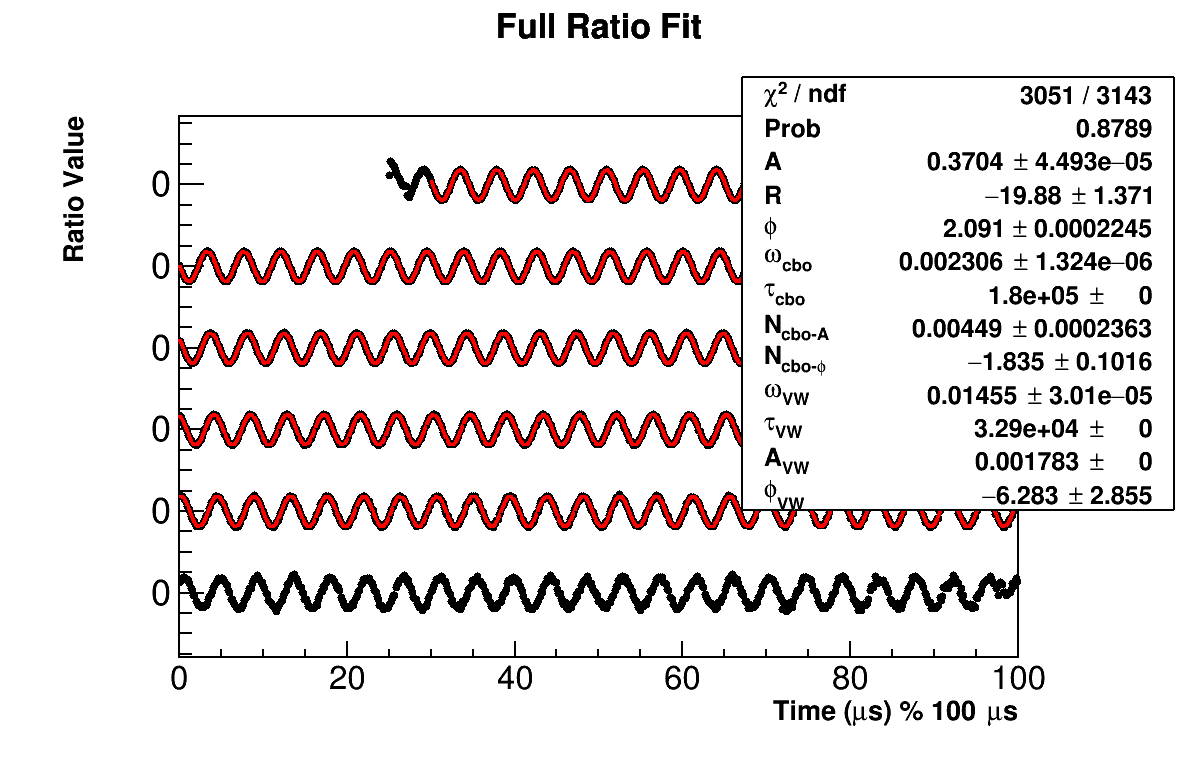
\includegraphics[width=\textwidth]{ratioCBO_moduloPlot-VW}
	    \caption[VWModuloPlot]{Fit results with the VW term included. The VW parameters have been fixed to values determined from a T Method fit to the data. The x axis is in units of $\mu$s modulo 100 $\mu$s, with successive portions of the data points and fit shifted downwards on the plot. The fit ranges from $\SI{30.2}{\mu s}$ to $\SI{650}{\mu s}$.}
	    \label{fig:VWModuloPlot}
	\end{figure}



\section{Sensitivity of \texorpdfstring{$\omega_{a}$}{} to various effects}

	\subsection{\gmtwo Period Guess}
	\label{SubSec:gm2Guess}

		To perform the ratio method, the \gmtwo period needs to be known a priori to high precision. This is because this value is used when time shifting the individual counts before filling the ratio histograms. By scanning over various \gmtwo period guesses the dependence of R on $T_{a}$ can be determined, as shown in Figure \ref{fig:gm2PeriodGuess}. The systematic error can then be calculated as 
			\begin{align}
				\delta R_{period} = \delta\alpha_{period} \times \frac{dR}{d\alpha_{period}}
			\end{align}
		where $\delta\alpha_{period}$ is the uncertainty on $T_{a}$. 

		Since the period that the counts need to be shifted by is already modified by the hardware blinding, it is technically the hardware shifted \gmtwo period that we want to use. As described in \cite{ClockManual}, the calorimeter digitizers use a ``40'' MHz clock which has been blinded to a value in the range of 39.997 to 39.999 MHz. This corresponds to a 75 ppm range in the frequency we're after, in a uniform distribution. Calculating the uncertainty from said uniform distribution and adding it in quadrature with a conservative 10 ppm uncertainty in the guess on the true \gmtwo period: 
			\begin{align}
				\delta\alpha_{period} = \sqrt{(75)^{2}/12 + 10^{2}} = \SI{23.8}{ppm}
			\end{align}
		This results in a systematic error of $\SI{23.8}{ppm} \times \SI{1.16e-4}{ppm/ppm} = \SI{2.8}{ppb}$.

		\begin{figure}[]
			\centering
			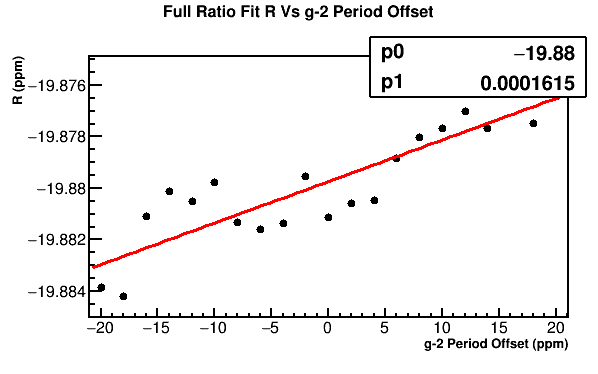
\includegraphics[width=.6\textwidth]{RatioCBO_R_Vs_gm2PeriodGuess_Canv}
		    \caption[gm2PeriodGuess]{Fitted R value as a function of the ppm level offset from the default guess used for the \gmtwo period, \ref{eq:Ta}. Error bars have been removed from this plot, otherwise it appears as a flat line. There appears to be a noticeable oscillation in the points at \gmtwo period guesses beyond the range of -25 ppm - +25 ppm, therefore the fit has been restricted to that range. The slope is .116 ppb per ppm offset in $T_{a}$.}
		    \label{fig:gm2PeriodGuess}
		\end{figure}

	\subsection{Lifetime used in weighting}
	\label{SubSec:LifetimeWeighting}

		Similarly to the \gmtwo period guesses used when constructing the time spectra for the ratio method, the lifetime of the muon is used when splitting the counts into the various histograms with different weights, as seen in Equation \ref{Eqn:Weighting}. To check for a systematic effect on R from getting this lifetime wrong, I scanned over a range of such lifetimes around the default value used, $\SI{64.4}{\mu s}$. As shown in Figure \ref{fig:weightingLifetime}, the slope is 4.015 ppb per $\mu$s. Since the uncertainty on the lifetime is much less than a microsecond, this systematic error is neglible.

		\begin{figure}[]
			\centering
			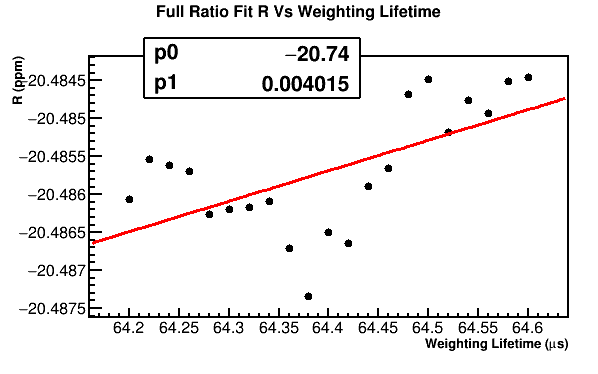
\includegraphics[width=.6\textwidth]{RatioCBO_R_Vs_weightingLifetime_Canv}
		    \caption[weightingLifetime]{Fitted R value as a function of the lifetime used in the weighting of counts into histograms. Error bars have been removed from this plot, otherwise it appears as a flat line. The slope is 4.015 ppb per $\mu$s.}
		    \label{fig:weightingLifetime}
		\end{figure}


	\subsection{Bin Width}

		The systematic uncertainty from the bin width, chosen to eliminate the fast rotation signal, was calculated by performing the histogramming and fitting stages with varying values of bin widths. The systematic uncertainty is taken as the RMS spread of the fitted R values. As shown in Figure \ref{fig:BinWidth} it is 44.5 ppb.

		\begin{figure}[]
			\centering
			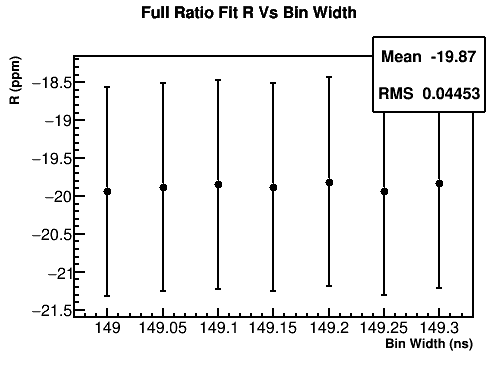
\includegraphics[width=.6\textwidth]{BinWidthComparison_R}
		    \caption[BinWidth]{Plotted are fitted R values for varying bin widths ranging from 149.00 ns to 149.30 ns in steps of 5 ns.}
		    \label{fig:BinWidth}
		\end{figure}

	\subsection{Randomization}
	\label{Sec:Randomization}

		In the histogramming phase of my analysis, random seeds are used in two places. One for the randomization of counts into the 4 separate datasets that go into the ratio, and one for the time randomization to reduce the fast rotation. It's necessary to make sure that results are consistent among random seeds, and that the final answer wasn't a particularly fortuitous or disastrous choice. In order to test this I performed fits with 50 different random seeds, the $\chi^{2}/NDF$ and fitted R values of which are plotted in Figure \ref{fig:RandomSeeds}. Results are consistent and very much within error of each other. I also performed fit start scans for a couple of the random seeds as an extra check to make sure the fitting was behaving consistently as shown in Figures \ref{fig:RandomSeedFitStartScansChi2} and \ref{fig:RandomSeedFitStartScansR}. I've included plots of the other fit parameters as a function of random seed in Figures \ref{fig:RandomSeedsPars1} - \ref{fig:RandomSeedsPars3}.

		\begin{figure}[]
		\centering
		    \begin{subfigure}[t]{0.45\textwidth}
			    \centering
				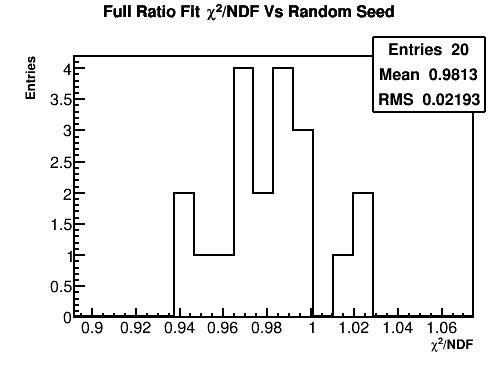
\includegraphics[width=\textwidth]{RatioCBO_Chi2NDF_Vs_Iter_Canv_hist}
			    \caption{$\chi^{2}$/NDF values for 50 random seeds. The mean is near 1.}
		    \end{subfigure}
		    \hspace{4mm}
		    \begin{subfigure}[t]{0.45\textwidth}
			    \centering
				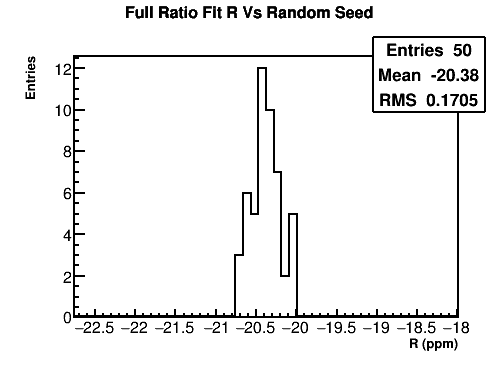
\includegraphics[width=\textwidth]{RatioCBO_R_Vs_Iter_Canv_hist}
			    \caption{R values for 50 random seeds. The mean is -20.38 ppm and the RMS is 170.5 ppb.}
			\label{Subfig:RVsRandomSeed}
		    \end{subfigure}% %you need this % here to add spacing between subfigures
		\caption[RandomSeeds]{Plotted are the $\chi^{2}$/NDF and fitted R values for 50 random seeds.}
		\label{fig:RandomSeeds}
		\end{figure}

		\begin{figure}[]
		\centering
		    \begin{subfigure}[t]{0.45\textwidth}
			    \centering
				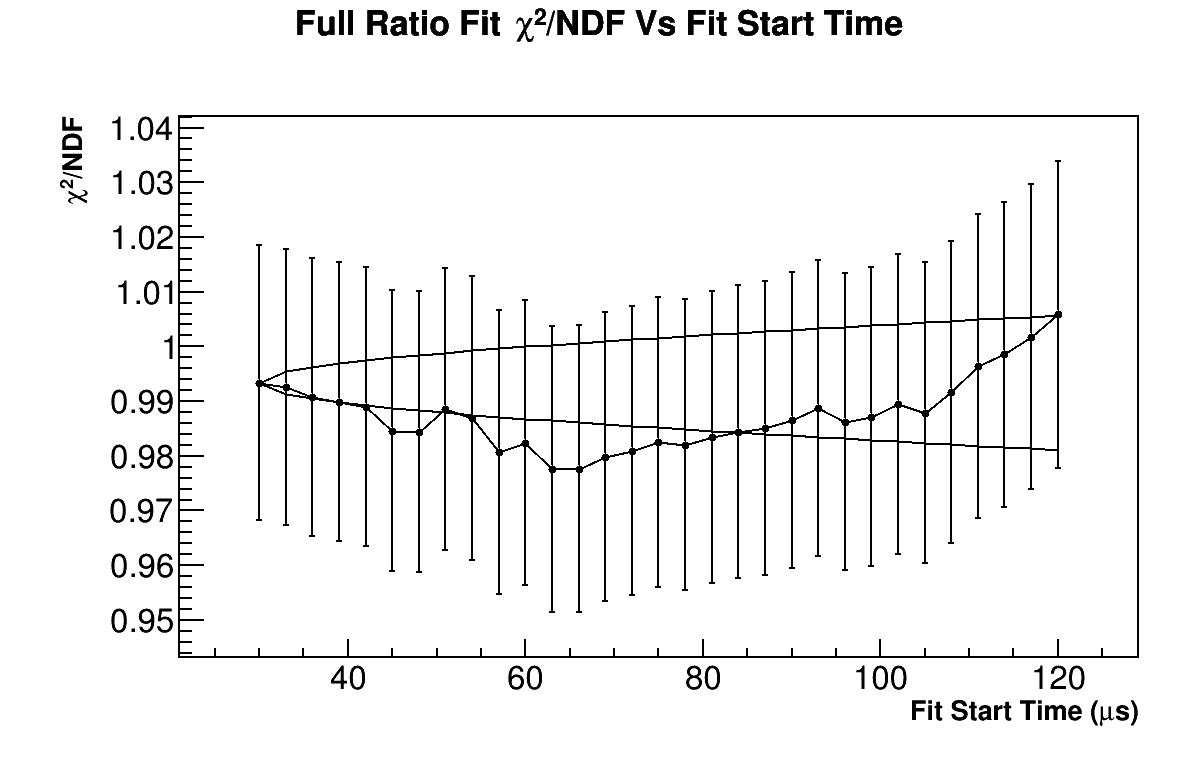
\includegraphics[width=\textwidth]{RatioCBO_Chi2NDF_Vs_FS_canv-Seed0}
			    \caption{Seed 1}
		    \end{subfigure}
		    \begin{subfigure}[t]{0.45\textwidth}
			    \centering
				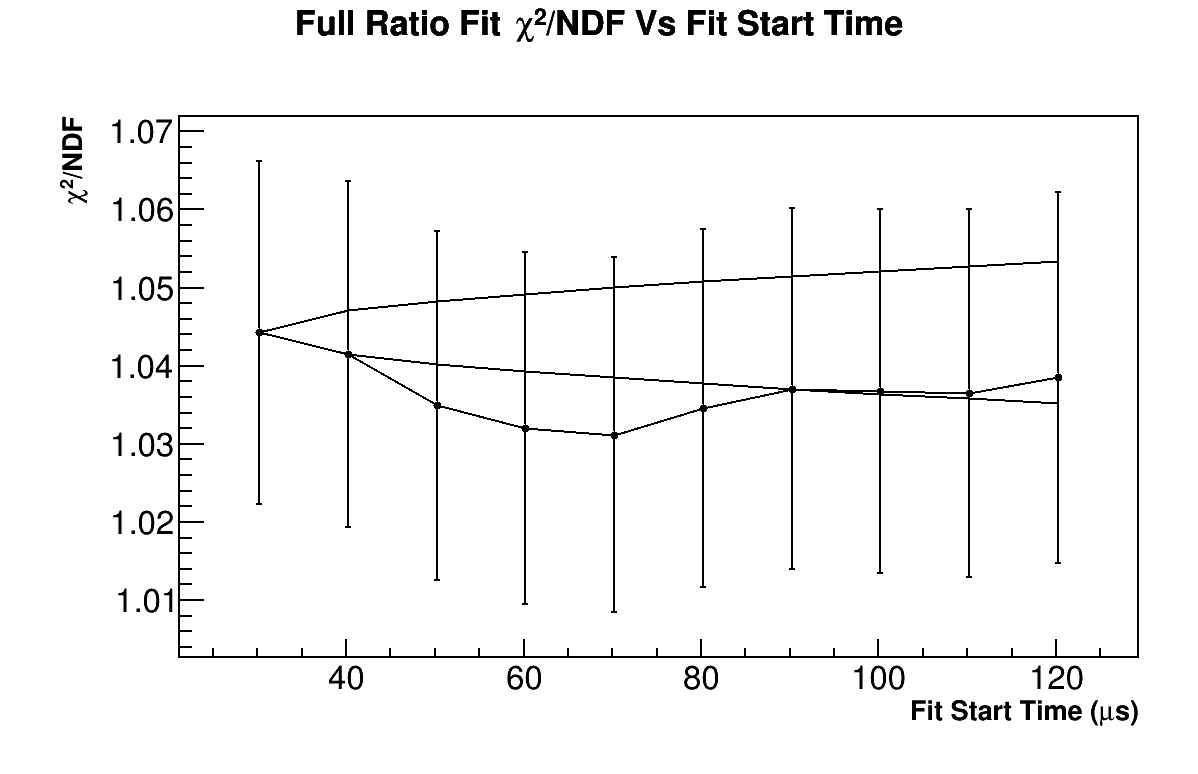
\includegraphics[width=\textwidth]{RatioCBO_Chi2NDF_Vs_FS_canv-Seed1}
			    \caption{Seed 2}
		    \end{subfigure}% %you need this % here to add spacing between subfigures
		    \vspace{4mm}
		    \begin{subfigure}[t]{0.45\textwidth}
			    \centering
				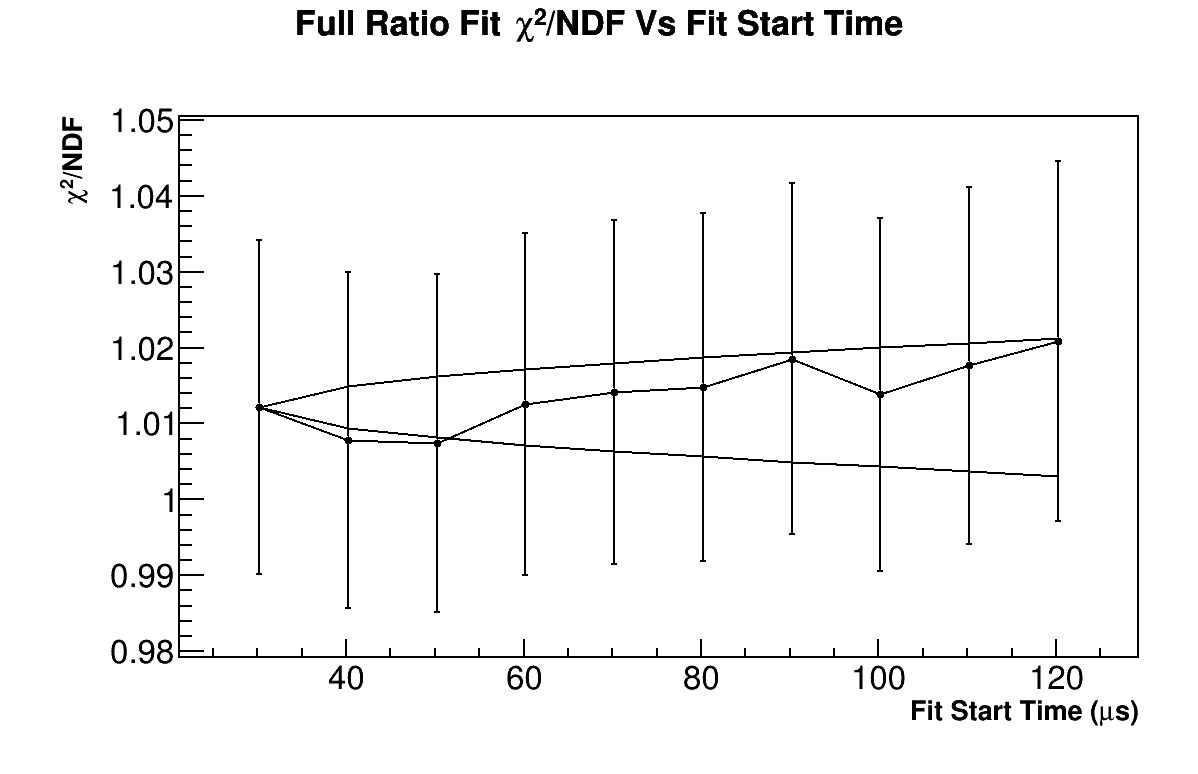
\includegraphics[width=\textwidth]{RatioCBO_Chi2NDF_Vs_FS_canv-Seed2}
			    \caption{Seed 3}
		    \end{subfigure}
		    \begin{subfigure}[t]{0.45\textwidth}
			    \centering
				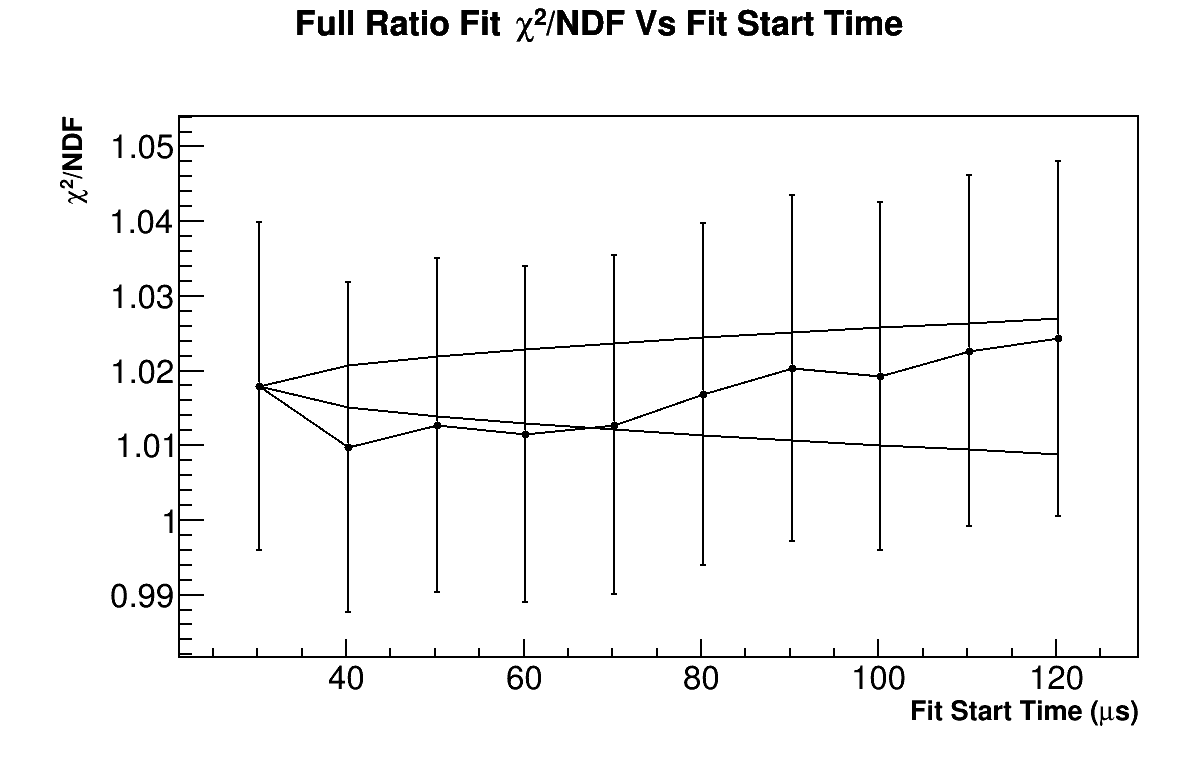
\includegraphics[width=\textwidth]{RatioCBO_Chi2NDF_Vs_FS_canv-Seed3}
			    \caption{Seed 4}
		    \end{subfigure}% %you need this % here to add spacing between subfigures
		\caption[RandomSeedFitStartScansChi2]{Fit start time scans for the \chisq for four random seeds of the randomization of the same dataset. Compare to Figure \ref{fig:Chi2FSScan}. The general behaviour of the fits vs fit start time is consistent and relatively the same, but as is seen the scans can rise and fall at different points due to the choice of randomization.}
		\label{fig:RandomSeedFitStartScansChi2}
		\end{figure}

		\begin{figure}[]
		\centering
		    \begin{subfigure}[t]{0.45\textwidth}
			    \centering
				\includegraphics[width=\textwidth]{RatioCBO_R_FS_canv-Seed0}
			    \caption{Seed 1}
		    \end{subfigure}
		    \begin{subfigure}[t]{0.45\textwidth}
			    \centering
				\includegraphics[width=\textwidth]{RatioCBO_R_FS_canv-Seed1}
			    \caption{Seed 2}
		    \end{subfigure}% %you need this % here to add spacing between subfigures
		    \vspace{4mm}
		    \begin{subfigure}[t]{0.45\textwidth}
			    \centering
				\includegraphics[width=\textwidth]{RatioCBO_R_FS_canv-Seed2}
			    \caption{Seed 3}
		    \end{subfigure}
		    \begin{subfigure}[t]{0.45\textwidth}
			    \centering
				\includegraphics[width=\textwidth]{RatioCBO_R_FS_canv-Seed3}
			    \caption{Seed 4}
		    \end{subfigure}% %you need this % here to add spacing between subfigures
		\caption[RandomSeedFitStartScansR]{Fit start time scans for the fitted R parameter for four random seeds of the randomization of the same dataset. The general behaviour of the R value vs fit start time is very consistent between seeds.}
		\label{fig:RandomSeedFitStartScansR}
		\end{figure}

		If the reported final answer on R is that of a single fit, then I believe there should be no systematic error on R due to the randomization. Such an error should be contained within the statistical error of the fitted parameter. If however the reported final answer is the average R value from many random seeds, then I can see why one might want to add in such a systematic error. For the latter case I calculate the systematic error on R as:
			\begin{align}
				\delta R_{rand} = \sigma(R)/\sqrt{N-1},
			\label{Eqn:Rand}
			\end{align}
		where $\sigma(R)$ is the RMS spread in R and N is the number of random seeds fitted, in this case 50. Therefore with an RMS on R of 170.5 ppb, the systematic error on the average R due to the randomization is 24.4 ppb. Perhaps the best thing to do is to report the fitted R value from a single fit that is closest to the mean, to avoid this error entirely while remaining closest to the average value.

		\begin{figure}[]
		\centering
		    \begin{subfigure}[t]{0.45\textwidth}
			    \centering
				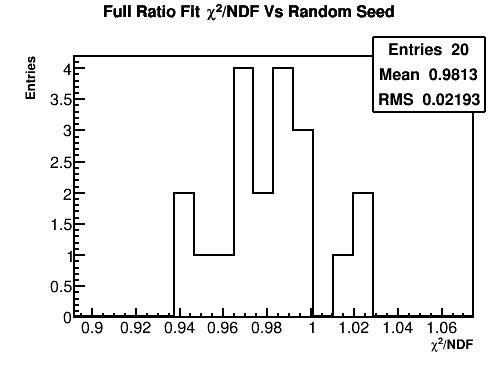
\includegraphics[width=\textwidth]{RatioCBO_Chi2NDF_Vs_Iter_Canv_hist}
			    \caption{$\chi^{2}$/NDF}
		    \end{subfigure}
		    \hspace{4mm}
		    \begin{subfigure}[t]{0.45\textwidth}
			    \centering
				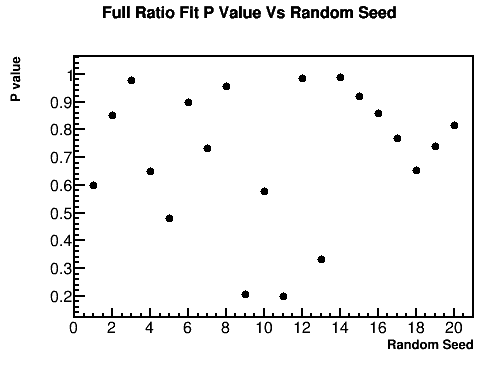
\includegraphics[width=\textwidth]{RatioCBO_PVal_Vs_Iter_Canv}
			    \caption{P value}
		    \end{subfigure}% %you need this % here to add spacing between subfigures
		   	\vspace{4mm}
		    \begin{subfigure}[t]{0.45\textwidth}
			    \centering
				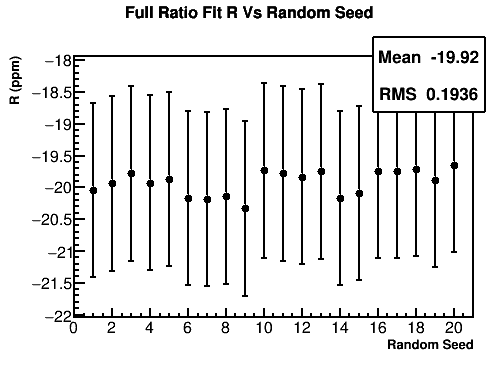
\includegraphics[width=\textwidth]{RatioCBO_R_Vs_Iter_Canv}
			    \caption{R in graph format.}
		    \end{subfigure}
		    \hspace{4mm}
		    \begin{subfigure}[t]{0.45\textwidth}
			    \centering
				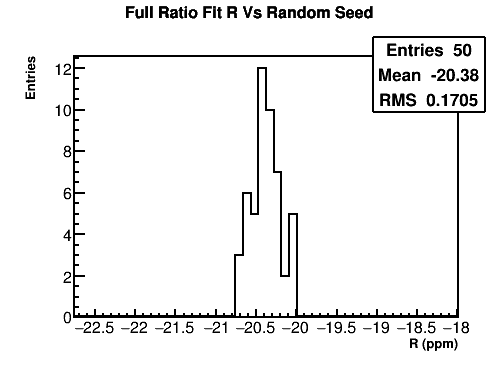
\includegraphics[width=\textwidth]{RatioCBO_R_Vs_Iter_Canv_hist}
			    \caption{R in histogram format.}
		    \end{subfigure}% %you need this % here to add spacing between subfigures
		\caption[RandomSeedsPars1]{Plotted are various fitted parameters for 50 different random seeds in graph and histogram format.}
		\label{fig:RandomSeedsPars1}
		\end{figure}

		\begin{figure}[]
		\centering
		    \begin{subfigure}[t]{0.45\textwidth}
			    \centering
				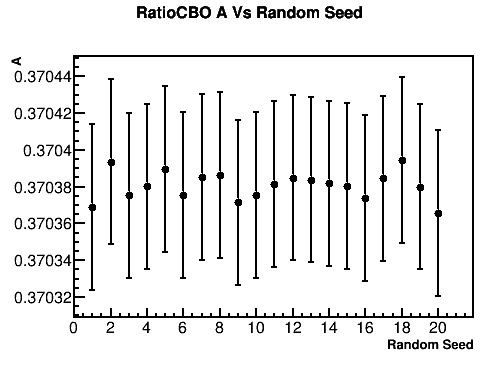
\includegraphics[width=\textwidth]{RatioCBO_A_Vs_Iter_Canv}
			    \caption{A in graph format.}
		    \end{subfigure}
		    \hspace{4mm}
		    \begin{subfigure}[t]{0.45\textwidth}
			    \centering
				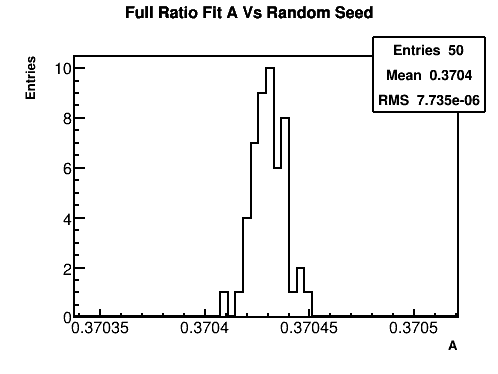
\includegraphics[width=\textwidth]{RatioCBO_A_Vs_Iter_Canv_hist}
			    \caption{A in histogram format.}
		    \end{subfigure}% %you need this % here to add spacing between subfigures
		   	\vspace{4mm}
		    \begin{subfigure}[t]{0.45\textwidth}
			    \centering
				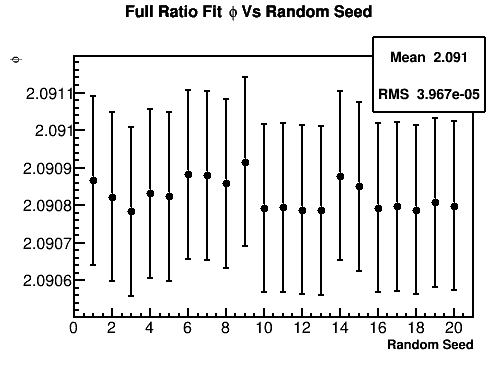
\includegraphics[width=\textwidth]{RatioCBO_phi_Vs_Iter_Canv}
			    \caption{\gmtwo phase in graph format.}
		    \end{subfigure}
		    \hspace{4mm}
		    \begin{subfigure}[t]{0.45\textwidth}
			    \centering
				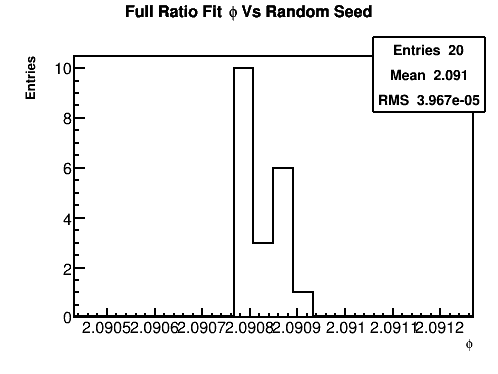
\includegraphics[width=\textwidth]{RatioCBO_phi_Vs_Iter_Canv_hist}
			    \caption{\gmtwo phase in histogram format.}
		    \end{subfigure}% %you need this % here to add spacing between subfigures
		   	\vspace{4mm}
		   	\begin{subfigure}[t]{0.45\textwidth}
			    \centering
				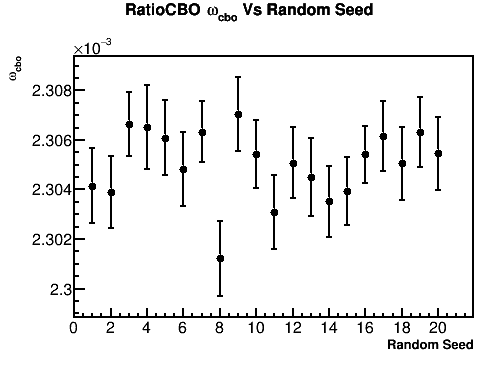
\includegraphics[width=\textwidth]{RatioCBO_omega_cbo_Vs_Iter_Canv}
			    \caption{CBO frequency in graph format.}
		    \end{subfigure}
		    \hspace{4mm}
		    \begin{subfigure}[t]{0.45\textwidth}
			    \centering
				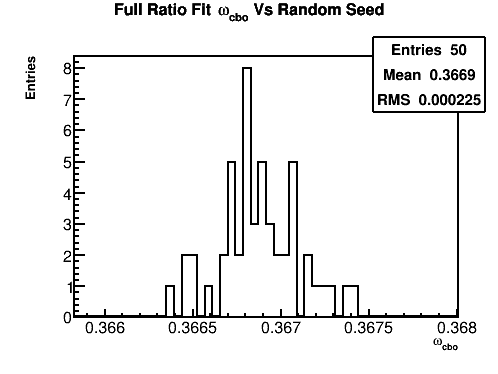
\includegraphics[width=\textwidth]{RatioCBO_omega_cbo_Vs_Iter_Canv_hist}
			    \caption{CBO frequency in histogram format.}
		    \end{subfigure}% %you need this % here to add spacing between subfigures
		\caption[RandomSeedsPars2]{Plotted are various fitted parameters for 50 different random seeds in graph and histogram format.}
		\label{fig:RandomSeedsPars2}
		\end{figure}

		\begin{figure}[]
		\centering
		    \begin{subfigure}[t]{0.45\textwidth}
			    \centering
				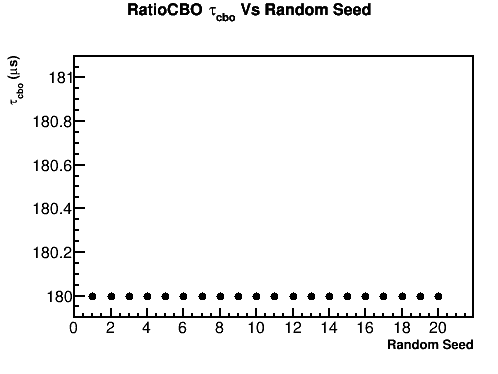
\includegraphics[width=\textwidth]{RatioCBO_tau_cbo_Vs_Iter_Canv}
			    \caption{CBO lifetime in graph format.}
		    \end{subfigure}
		    \hspace{4mm}
		    \begin{subfigure}[t]{0.45\textwidth}
			    \centering
				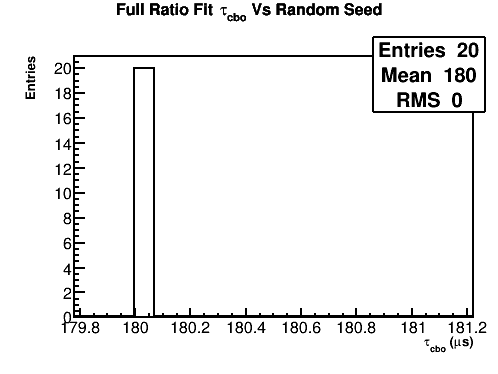
\includegraphics[width=\textwidth]{RatioCBO_tau_cbo_Vs_Iter_Canv_hist}
			    \caption{CBO lifetime in histogram format.}
		    \end{subfigure}% %you need this % here to add spacing between subfigures
		   	\vspace{4mm}
		    \begin{subfigure}[t]{0.45\textwidth}
			    \centering
				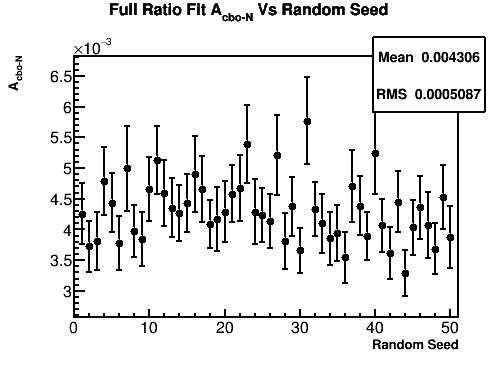
\includegraphics[width=\textwidth]{RatioCBO_A_cbo-N_Vs_Iter_Canv}
			    \caption{CBO N amplitude in graph format.}
		    \end{subfigure}
		    \hspace{4mm}
		    \begin{subfigure}[t]{0.45\textwidth}
			    \centering
				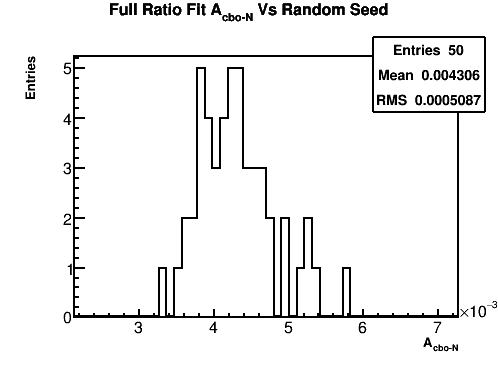
\includegraphics[width=\textwidth]{RatioCBO_A_cbo-N_Vs_Iter_Canv_hist}
			    \caption{CBO N amplitude in histogram format.}
		    \end{subfigure}% %you need this % here to add spacing between subfigures
		   	\vspace{4mm}
		   	\begin{subfigure}[t]{0.45\textwidth}
			    \centering
				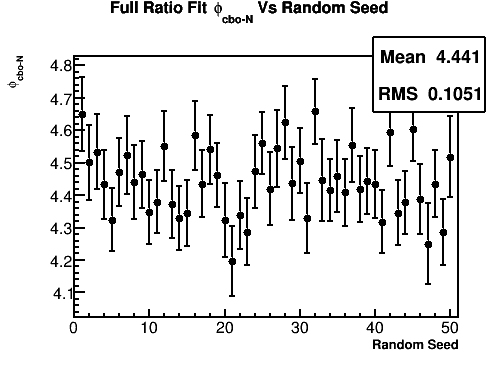
\includegraphics[width=\textwidth]{RatioCBO_phi_cbo-N_Vs_Iter_Canv}
			    \caption{CBO N phase in graph format.}
		    \end{subfigure}
		    \hspace{4mm}
		    \begin{subfigure}[t]{0.45\textwidth}
			    \centering
				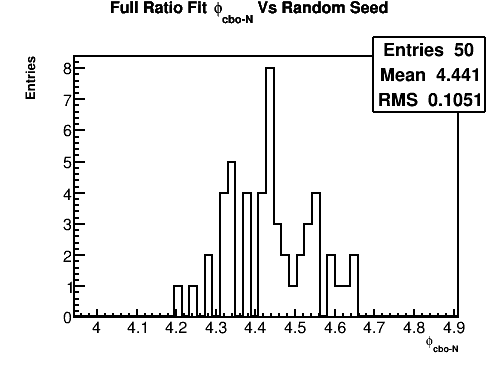
\includegraphics[width=\textwidth]{RatioCBO_phi_cbo-N_Vs_Iter_Canv_hist}
			    \caption{CBO N phase in histogram format.}
		    \end{subfigure}% %you need this % here to add spacing between subfigures
		\caption[RandomSeedsPars3]{Plotted are various fitted parameters for 50 different random seeds in graph and histogram format.}
		\label{fig:RandomSeedsPars3}
		\end{figure}


	\subsection{Bunch Number}

		Each fill during normal data taking comes from one of eight separate muon bunches. Each individual bunch, due to the nature of the particle production and upstream beamline effects, likely has separate properties. In order to explore this the fit results can be examined as a function of bunch number. The fit results are shown in Figures \ref{fig:BunchNumChi2}, \ref{fig:BunchNumPars}, and \ref{fig:BunchNumParsCBO}. As can be seen in the first figure, it appears that the goodness-of-fit as a function of bunch number is not quite adequate, with most points being above 1. The fitted parameter values for the different bunches shown in the latter figures appear for the most part consistent, with some clear differences between the different bunches. This is especially evident in Figure \ref{SubFig:gm2PhaseBunch}, where the \gmtwo phase is clearly different between bunches. This could potentially lead to a systematic error on R, for example due to different lost muon characteristics per bunch and thus a changing average \gmtwo phase over the course of a fill. It is nice to see however that the average R value and \gmtwo phases between the different bunches are very consistent with the results from the bunch sum fit. The other parameters are all consistent as well to different degrees. This is only a cursory look at the analysis results on a per bunch basis, and the systematic effects on R (if indeed there are any) have yet to be explored in any great detail.

		\begin{figure}[]
			\centering
			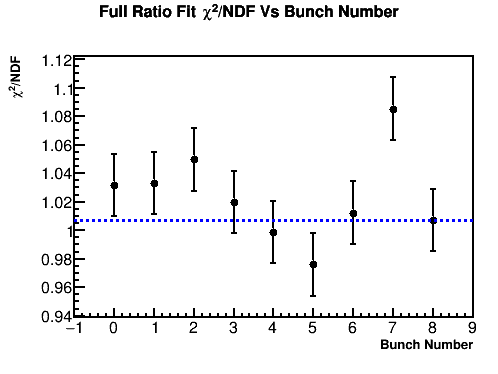
\includegraphics[width=.6\textwidth]{RatioCBO_Chi2NDF_Vs_BunchNum_Canv}
		    \caption[BunchNumChi2]{Plotted are \chisq per degree of freedom values for the different bunch numbers. The point at bunch number 8 is the fit result from all bunches added together. The blue dashed line is set at the added bunch number result.}
		    \label{fig:BunchNumChi2}
		\end{figure}

		\begin{figure}[]
		\centering
		    \begin{subfigure}[t]{0.4\textwidth}
			    \centering
				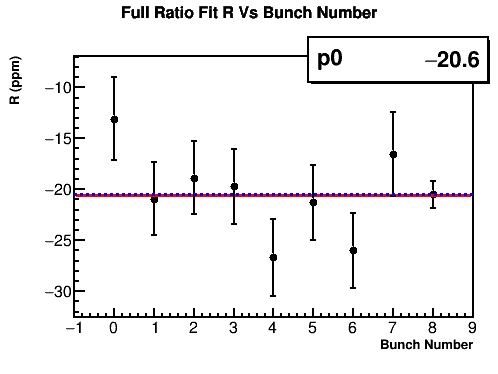
\includegraphics[width=\textwidth]{RatioCBO_R_Vs_BunchNum_Canv}
			    \caption{Fitted R values as a function of bunch number.}
		    \end{subfigure}
		    \hspace{4mm}
		    \begin{subfigure}[t]{0.4\textwidth}
			    \centering
				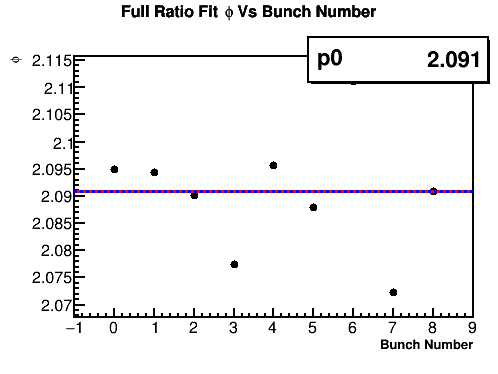
\includegraphics[width=\textwidth]{RatioCBO_phi_Vs_BunchNum_Canv}
			    \caption{Fitted \gmtwo phase values as a function of bunch number.}
			    \label{SubFig:gm2PhaseBunch}
		    \end{subfigure}% %you need this % here to add spacing between subfigures
			\vspace{4mm}
		    \begin{subfigure}[t]{0.4\textwidth}
			    \centering
				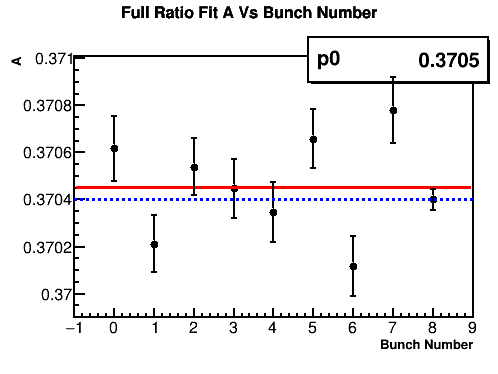
\includegraphics[width=\textwidth]{RatioCBO_A_Vs_BunchNum_Canv}
			    \caption{Fitted A values as a function of bunch number.}
		    \end{subfigure}
		\caption[BunchNumPars]{Plotted are the main fitted parameter values for the different bunch numbers. The point at bunch number 8 is the fit result from all bunches added together. The blue dashed line is set at the added bunch number result, and the red line is the fit to the individual bunches excluding the final point.}
		\label{fig:BunchNumPars}
		\end{figure}

		\begin{figure}[]
		\centering
		    \begin{subfigure}[t]{0.4\textwidth}
			    \centering
				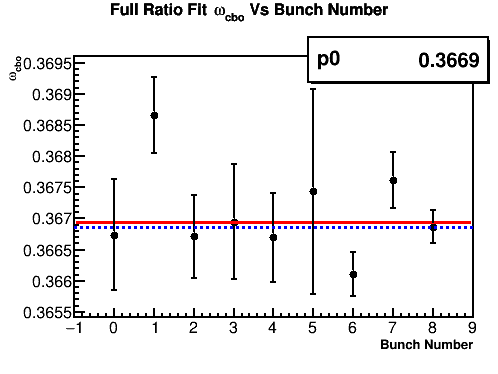
\includegraphics[width=\textwidth]{RatioCBO_omega_cbo_Vs_BunchNum_Canv}
			    \caption{Fitted CBO frequency values as a function of bunch number.}
		    \end{subfigure}
		    \hspace{4mm}
		    \begin{subfigure}[t]{0.4\textwidth}
			    \centering
				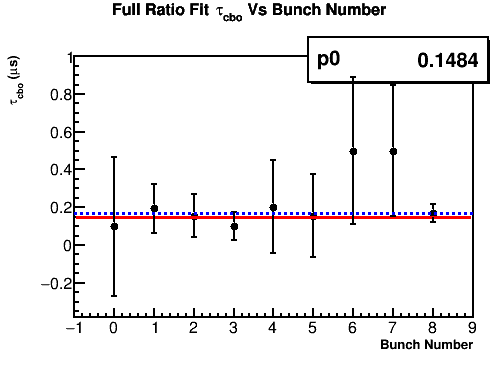
\includegraphics[width=\textwidth]{RatioCBO_tau_cbo_Vs_BunchNum_Canv}
			    \caption{Fitted CBO lifetime values as a function of bunch number. Bunches 6 and 7 hit the upper fit limit of $\SI{500}{\mu s}$.}
		    \end{subfigure}% %you need this % here to add spacing between subfigures
			\vspace{4mm}
		    \begin{subfigure}[t]{0.4\textwidth}
			    \centering
				\includegraphics[width=\textwidth]{RatioCBO_phi_cbo-N_Vs_BunchNum_Canv}
			    \caption{Fitted CBO phase values as a function of bunch number.}
		    \end{subfigure}
		    \hspace{4mm}
		    \begin{subfigure}[t]{0.4\textwidth}
			    \centering
				\includegraphics[width=\textwidth]{RatioCBO_A_cbo-N_Vs_BunchNum_Canv}
			    \caption{Fitted CBO N amplitude values as a function of bunch number.}
		    \end{subfigure}% %you need this % here to add spacing between subfigures
			\vspace{4mm}
		\caption[BunchNumParsCBO]{Plotted are the fitted CBO parameter values for the different bunch numbers. Some of the fitted parameters have large error bars, indicating that the fit had trouble fitting the CBO parameters. The point at bunch number 8 is the fit result from all bunches added together. The blue dashed line is set at the added bunch number result, and the red line is the fit to the individual bunches excluding the final point.}
		\label{fig:BunchNumParsCBO}
		\end{figure}


\clearpage

\section{Final Systematic Uncertainty Table}

The calculated systematic errors for the 60H dataset are shown in Table \ref{Tab:Systematics}. As a reminder, not all systematic uncertainty evaluations are fully completed. Here we see that...


\begin{table}[H]
\centering
\setlength\tabcolsep{10pt}
\renewcommand{\arraystretch}{1.2}
\begin{tabular*}{.5\linewidth}{@{\extracolsep{\fill}}|lG|}
  \hline
  	\multicolumn{2}{|c|}{\textbf{Summary of Systematic Errors}} \\
  \hline\hline
    Systematic Error 		& \multicolumn{1}{c|}{\SI{60}{H}} \\
  \hline
	Gain 			 		&  7.2   \\
	Pileup     	     		&  37.5  \\
	Lost Muons*             &  29.9  \\
	CBO      		 		&    \\
	VW 			     		&  \multicolumn{1}{c|}{$<1$} \\
	Bin Width        		&    \\
	Randomization    		&  24.4  \\
	% Bunch Number     		&        \\
	Other* 				  	&  2.8   \\
  \hline\hline		
  	Total   	     		&    \\
  \hline
\end{tabular*}
\caption{Systematic error table for the 60H dataset. All units are in ppb. The `*'s indicate that significant work still needs to be done in the error estimation. The lack of a `*' does not preclude future work on the rest of the systematic errors. }
\label{Tab:Systematics}
\end{table}






